\section{Design Goals}
Students were required to choose an appropriate internal clock frequency as
defined by the instructor-provided resources.  Once a frequency was chosen,
students used the chart provided in the ADC's datasheet~(reproduced in
Figure~\ref{f:element_chart}) to choose relevant component values.
%
\begin{figure}[H]
\centering
	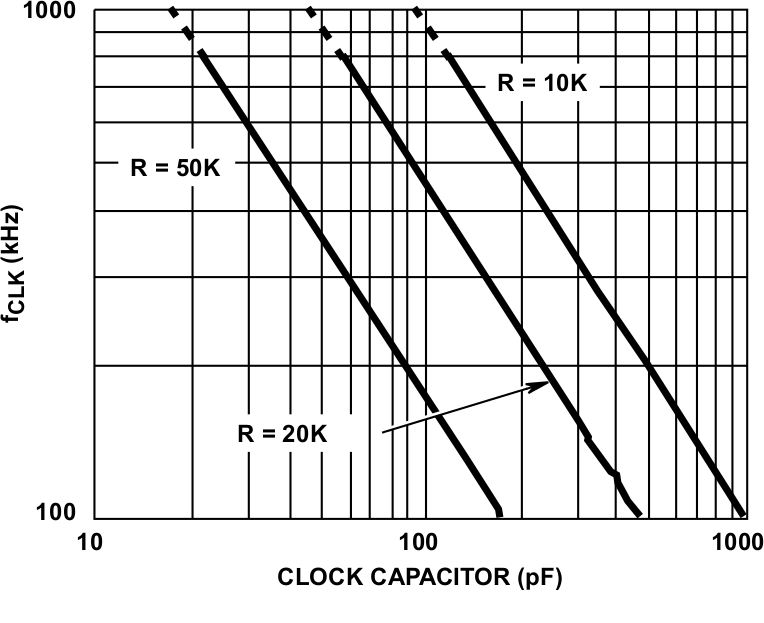
\includegraphics[width=.8\textwidth]{img/shot/ADC0804.png}
	\parbox{.8\textwidth}{
	\caption[Clock frequency element selection]{Chart provided by the Harris
	ADC0804 datasheet (also provided in the lab resources) to assist in the
	selection of elements for an arbitrary clock frequency.}
	\label{f:element_chart}}
\end{figure}
%
The student decided upon an internal clock frequency of~\SI{730}{\kilo\hertz}.
By Figure~\ref{f:element_chart}, he also chose to use a~\SI{10}{\kilo\ohm}
resistor and~\SI{\approx150}{\pico\farad}.  After obtaining appropriate
elements, the measured values were as listed in Table~\ref{t:elements}.
%
\begin{table}[H]
\centering
	\section{Elements}

After consulting the datasheet for the DAC0808 integrated circuit, it was
determined that three~\SI{5}{\kilo\ohm} resistors were required for the proper
operation of the chip.  The measured values are shown in
Table~\ref{t:elements}, along with the elements used in the construction of the
ADC in step 2 (which utilized the ADC0804 IC).
%
\begin{table}[H]
\centering
	\section{Elements}

After consulting the datasheet for the DAC0808 integrated circuit, it was
determined that three~\SI{5}{\kilo\ohm} resistors were required for the proper
operation of the chip.  The measured values are shown in
Table~\ref{t:elements}, along with the elements used in the construction of the
ADC in step 2 (which utilized the ADC0804 IC).
%
\begin{table}[H]
\centering
	\section{Elements}

After consulting the datasheet for the DAC0808 integrated circuit, it was
determined that three~\SI{5}{\kilo\ohm} resistors were required for the proper
operation of the chip.  The measured values are shown in
Table~\ref{t:elements}, along with the elements used in the construction of the
ADC in step 2 (which utilized the ADC0804 IC).
%
\begin{table}[H]
\centering
	\input{tbl/elements.tex}
	\parbox{.8\textwidth}{
	\caption[List of used elements]{Required, nominal, and measured element
	values used in the ADC and DAC circuits.}
	\label{t:elements}}
\end{table}
%
With errors for the DAC resistors all falling under~\SI{1}{\percent}, the
elements are all appropriately accurate for this application.

	\parbox{.8\textwidth}{
	\caption[List of used elements]{Required, nominal, and measured element
	values used in the ADC and DAC circuits.}
	\label{t:elements}}
\end{table}
%
With errors for the DAC resistors all falling under~\SI{1}{\percent}, the
elements are all appropriately accurate for this application.

	\parbox{.8\textwidth}{
	\caption[List of used elements]{Required, nominal, and measured element
	values used in the ADC and DAC circuits.}
	\label{t:elements}}
\end{table}
%
With errors for the DAC resistors all falling under~\SI{1}{\percent}, the
elements are all appropriately accurate for this application.

	\parbox{.6\textwidth}{
	\caption[Measured element values]{Required, nominal, and measured values
	for the ADC clock frequency elements.}
	\label{t:elements}}
\end{table}
%
As is shown, these elements are very close to the required element values.
This implies that the resulting clock frequency will be similarly close to the
chosen value of~\SI{730}{\kilo\hertz}.
